\subsection{MapBeskrivelse}

På figur xxx herunder ses det endelige layout af spillets map som det er blevet implementeret. 
Spillets map består af 20 rum, som indeholder forskellige artefakter.  
Det første rum, rum 1, indeholder spillets spawnpoint, markeret med X, hvor spillet starter.  
De resterende 19 rum indeholder en række udfordringer, i form af fjender som skal overvindes, samt hjælp til dette i form af forskellige genstande. 
Der er i alt fem fjender på banen, fire svagere fjender markeret E, og en boss markeret B. 
Der findes to forskellige slags genstande som skal hjælp spilleren på sin vej, våben(W) og skjold(S).  
Disse genstande henholdsvist forøger skaden man deler til fjender, og formindsker skade man tager. 
Bag bossen i rum 19, 
The Sword Of Destiny, markeret SOD, er placeret i rum 20 bag bossen. SOD er spillets endepunkt og når dette nåes, er spillet vundet.



\begin{figure}[H]
\centering
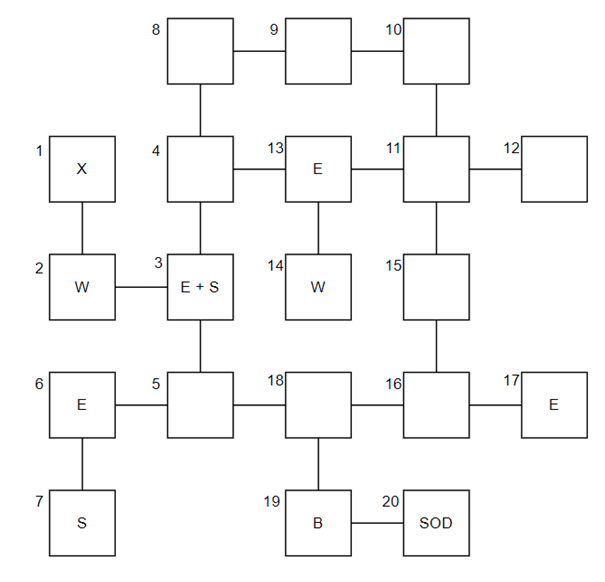
\includegraphics[width = 0.9\textwidth]{02-Body/Images/MapLayout.PNG}
\caption{Screenshot af final maplayout}
\label{fig:MapLayout-final}
\end{figure}